\documentclass{assignment}
\usepackage{amsmath}
\usepackage[ruled,vlined]{algorithm2e}
\usepackage{listings}
\usepackage{color}

\definecolor{dkgreen}{rgb}{0,0.6,0}
\definecolor{gray}{rgb}{0.5,0.5,0.5}
\definecolor{mauve}{rgb}{0.58,0,0.82}

\lstset{frame=tb,
  language=Python,
  aboveskip=3mm,
  belowskip=3mm,
  showstringspaces=false,
  columns=flexible,
  basicstyle={\small\ttfamily},
  numbers=none,
  numberstyle=\tiny\color{gray},
  keywordstyle=\color{blue},
  commentstyle=\color{dkgreen},
  stringstyle=\color{mauve},
  breaklines=true,
  breakatwhitespace=true,
  tabsize=3
}

%\coursetitle{Creating assignments}
%more class  https://ctan.org/topic/class
%more template https://www.latexstudio.net/
\courselabel{Stochastic Process}
\exercisesheet{Home Work 9}{Documentation}
\student{Pan Meng}
\semester{Fall 2021}
\date{Dec 30, 2021}
\finishdate{Dec 28, 2021}
%\usepackage[pdftex]{graphicx}
%\usepackage{subfigure}
\SetKw{KwBy}{by}
\begin{document}
% 根据输入的第一个参数围来读取图片显示的写法
\logo{logo.jpg}
% 固定死是logo.jpg的写法
% \logo

\begin{problemlist}
\pbitem 
A Manufacturer at each time period receives an order for 
her product with probability $p$ and receives no order with 
probability $1-p$.
At any period, she has a choice of processing all the unfilled orders 
in a batch, or process no order at all. The maximum number of orders that 
can remain unfilled is $n$.
The cost per unfilled order at each time period is $c > 0$, 
the setup cost to process the unfilled orders is $K > 0$.
The manufacturer wants to find a processing policy that minimizes 
the total expected cost with discount factor $\alpha<1$

\begin{problem}
\begin{answer}
  \vspace{-1cm}
\begin{flushleft}
  \large\textbf{1. model formulation}
\end{flushleft}
\begin{figure}[htb]
  \centering
  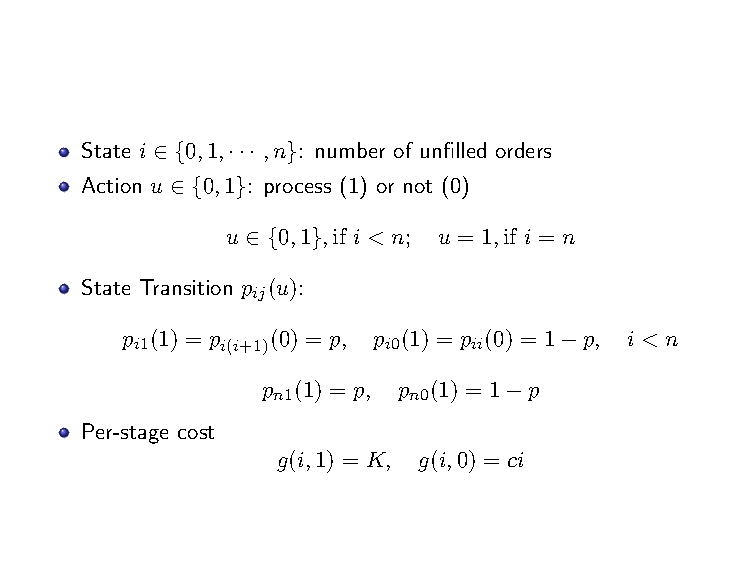
\includegraphics[width=0.7\linewidth]{figure/formulation.pdf}
  \caption{The formulation of Batch Manufacturing problem}
\end{figure}

\begin{flushleft}
  \large\textbf{2. pseudocode}
\end{flushleft}

\begin{algorithm}[h]
  \caption{Value Iteration}
  \KwIn{$c, K, n, p, u, \alpha$}
	\KwOut{policy,convergeed $J_θ^*$}  
	\BlankLine
	Initialize $\theta=0.001, \delta=\inf$;
	
	\While{\textnormal{$\delta>\theta$}}
  {
    \For{$i=0$ \KwTo $n$}
    {
      $$J_{K+1}(i)=min⁡(k+\alpha(1-p) J_K (0)+\alpha pJ_K (1),c i+\alpha(1-p) J_k (i)+\alpha pJ_k (i+1)$$
			$$δ=\lvert J_{K+1} (i)-J_K (i) \rvert$$

      }
	}
    \For{$i=0$ \KwTo $n$}
    {$$policy_{i} = argmin_{u\in U} (i+\alpha(1-p) J_K (i)+\alpha p J_k (i+1))$$}

\end{algorithm}

\begin{algorithm}[h]
  \caption{Policy Iteration}
  \KwIn{$c, K, n, p, u, \alpha, s$}
	\KwOut{policy,converged $J_θ^*$}  
	\BlankLine
	Initialize $\theta=0.001, \delta=\inf, s=0$;
	
	\While{\textnormal{$\delta>\theta$}}
  {
    \For{$i=0$ \KwTo $n$}
    {
      $$value_{expected}=0$$ \\
    
      $$value_{expercted}=\sum_{u\in U}p_u (K +\alpha \sum_{s\in S}J_k (i)$$

      }
	}

    \For{$i=0$ \KwTo $n$}
    {
      $$policy_{i}= argmin_{u∈U} (i+\alpha(1-p) J_k (i)+\alpha pJ_k (i+1))$$}
\end{algorithm}

\begin{flushleft}
  \large\textbf{3. code}
\end{flushleft}
\begin{lstlisting}
  class DiscountProblem():

    def __init__(self, c, K, n, p, a):
        self.c = c
        self.K = K
        self.n = n
        self.p = p
        self.a = a
        self.action_prob = {0: 0.5, 1: 0.5}
        self.transition = self.__init_transition()
        self.V = [0 for _ in range(n + 1)]

    def __init_transition(self):
        state_action = {}
        for i in range(self.n + 1):
            if (i == self.n):
                state_action[self.n] = {1: {1: self.p, 0: 1 - self.p}}
                continue
            state_action[i] = {1: {0: 1 - self.p, 1: self.p}, 0: {i + 1: self.p, i: 1 - self.p}}
        return state_action

    def next_best_action(self, s, V):
        action_values = np.zeros(2)
        for a in self.transition[s]:
            for state in self.transition[s][a]:
                cost = self.K if a == 1 else self.c * s
                action_values[a] += self.transition[s][a][state] * (cost + self.a * V[state])
        return np.argmin(action_values), np.min(action_values)

    def value_Iteration(self):
        THETA = 0.0001
        delta = float("inf")
        round_num = 0

        while delta > THETA:
            print(delta)
            delta = 0
            print("\nValue Iteration: Round " + str(round_num))
            for s in range(self.n + 1):
                best_action, best_action_value = self.next_best_action(s, self.V)
                delta = max(delta, np.abs(best_action_value - self.V[s]))
                self.V[s] = best_action_value

            print(delta)
            round_num += 1

        policy=[]
        for s in range(self.n + 1):
            best_action, best_action_value = self.next_best_action(s, self.V)
            policy.append(best_action)
        return policy

    def __policy_evaluation(self):
        V = np.zeros(self.n+1)
        THETA = 0.0001
        delta = float("inf")

        while delta > THETA:
            delta = 0
            for s in range(self.n+1):
                expected_value = 0
                for a in self.transition[s]:
                    for state in self.transition[s][a]:
                        cost = self.K if a == 1 else self.c * s
                        expected_value += 0.5*self.transition[s][a][state] * (cost + self.a * V[state])
                delta = max(delta, np.abs(V[s] - expected_value))
                V[s] = expected_value
        return V

    def policy_iteration(self):
        policy = np.tile(np.eye(2)[1], (self.n+1, 1))

        is_stable = False

        round_num = 0

        while not is_stable:
            is_stable = True

            print("\nRound Number:" + str(round_num))
            round_num += 1

            print("Current Policy")

            V = self.__policy_evaluation()

            for s in range(self.n+1):
                action_by_policy = np.argmax(policy[s])
                best_action, best_action_value = self.next_best_action(s, V)
                # print("\nstate=" + str(s) + " action=" + str(best_action))
                policy[s] = np.eye(2)[best_action]
                if action_by_policy != best_action:
                    is_stable = False

        policy = [np.argmax(policy[s]) for s in range(self.n+1)]
        return policy
  \end{lstlisting}
%\begin{table}[htb]
%    \begin{tabular}{c|c|c|c|c|c|c}
%        \hline
%       $u_0$&-5&-4&-3&-2&-1&0 \\ 
%       
%       $x_0$& 5& 5& 5& 5& 5&5 \\
%         k=0& 34 & 34& 34& 34& 34& 34 \\
%       \hline
%       $x_1$& 2& 2& 2& 2& 2& 2 \\
%       $u_1$& -1& -1& -1& -1& -1& -1 \\
%         k=1& 39 & 39& 39& 39& 39& 39 \\
%       \hline
%       $x_2$& 1& 1& 1& 1& 1& 1 \\
%       $u_2$& 0& 0& 0& 0& 0& 0 \\
%         k=2& 40 & 40& 40& 40& 40& 40 \\
%       \hline
%       $x_3$& 1& 1& 1& 1& 1& 1 \\
%       $u_3$& 0& 0& 0& 0& 0& 0 \\
%         k=3& 41& 41& 41& 41& 41& 41\\
%         \hline
%    \end{tabular}
%\end{table}

\begin{flushleft}
 \large \textbf{4. simulation experiment}
\end{flushleft}
Discounted Problem

input: 7 2 8 0.57 0.49

value iteration: 5 

strategy: [0, 1, 1, 1, 1, 1, 1, 0] 

policy iteration:38

strategy: [0, 1, 1, 1, 1, 1, 1, 0] 


\end{answer}
\end{problem}

%\pbitem What does the preamble contain ?



%The preamble may contain the following declarations\footnote{Current markup's preamble.} :

%\begin{verbatim}
%\documentclass{assignment}
%\coursetitle{Creating assignments}
%\courselabel{ASG 101}
%\exercisesheet{Home Work 1}{Documentation}
%\student{Madhusudan Singh}
%\semester{Summer 2004}
%\date{July 14, 2004}
%%\usepackage[pdftex]{graphicx}
%%\usepackage{subfigure}
%\end{verbatim}


%Its possible. Just pass the options in the preamble :

%\begin{verbatim}
%\documentclass[option1,option2, ...]{assignment}
%\end{verbatim}


%Equation numbers refer to the problem number. For instance,

%\begin{verbatim}
%\begin{eqnarray}
%E & = & mc^{2} \label{eqn:emc2} \\
%\textrm{That is how equations are numbered} \ldots \label{eqn:numbered} \\
%\textrm{Or not numbered} \ldots \nonumber
%\end{eqnarray}
%\end{verbatim}
%
%\begin{eqnarray}
%E & = & mc^{2} \label{eqn:emc2} \\
%\textrm{That is how equations are numbered} \ldots \label{eqn:numbered} \\
%\textrm{Or not numbered} \ldots \nonumber
%\end{eqnarray}




%\begin{verbatim}
%\begin{answer}
%\begin{eqnarray}
%Answer=f(bold) \nonumber
%\end{eqnarray}
%\end{answer}
%\end{problem}
%\end{verbatim}


%\pbitem Can one have more than one answer section for the problem ?
%
%\begin{problem}
%
%Most definitely.
%
%Certain problems have many parts :
%
%\begin{enumerate}
%\item Part 1
%
%\begin{answer}
%Answer to part one.
%\end{answer}
%
%\item Part 2
%
%\begin{answer}
%Answer to part two.
%\end{answer}
%
%\end{enumerate}
%
%\begin{verbatim}
%\begin{enumerate}
%\item Part 1
%
%\begin{answer}
%Answer to part one.
%\end{answer}
%
%\item Part 2
%
%\begin{answer}
%Answer to part two.
%\end{answer}
%
%\end{enumerate}
%
%\end{verbatim}
%
%\end{problem}
%
%
%\pbitem What are the copyright conditions for this class file ?
%
%\begin{problem}
%
%This material is subject to the \LaTeX\ Project Public License. See http://www.ctan.org/tex-archive/help/Catalogue/licenses.lppl.html for the details of that license. See the LICENSE file for more details.
%
%
%\begin{answer}
%\begin{eqnarray}
%&& Q. E. D. \nonumber
%\end{eqnarray}
%\end{answer}
%
%\end{problem}
%
%
%\pbitem How do I get help using this class ?
%\begin{problem}
%
%
%You may post your queries on comp.text.tex . I check it fairly regularly.
%\end{problem}

\end{problemlist}

\end{document}
